\documentclass[UTF8,a4paper,12pt,oneside]{ctexrep}

\usepackage{geometry}
\usepackage{setspace}
\usepackage{graphicx}
\usepackage{booktabs}
\usepackage{longtable}
\usepackage{tabularx}
\usepackage{array}
\usepackage{enumitem}
\usepackage{xcolor}
\usepackage{listings}
\usepackage{hyperref}
\usepackage{fancyhdr}
\usepackage{titlesec}
\usepackage{caption}
\usepackage{float}
\usepackage{tikz}
\usepackage{amsmath}
\usetikzlibrary{arrows.meta,positioning,fit,shapes.geometric}

\geometry{left=2.8cm,right=2.8cm,top=2.8cm,bottom=2.8cm}
\onehalfspacing
\setlength{\parindent}{2em}
\setlength{\parskip}{0.25em}
\setlist[itemize]{leftmargin=2.5em}
\setlist[enumerate]{leftmargin=2.7em}

\hypersetup{
  colorlinks=true,
  linkcolor=black,
  urlcolor=blue,
  citecolor=black,
  pdfauthor={seccomp-privacy-platform team},
  pdftitle={面向电商隐私分析场景的 SSE + PJC 平台设计与实现}
}

\pagestyle{fancy}
\setlength{\headheight}{15pt}
\fancyhf{}
\fancyhead[C]{面向电商隐私分析场景的 SSE + PJC 平台设计与实现}
\fancyfoot[C]{\thepage}
\renewcommand{\headrulewidth}{0.4pt}

\ctexset{
  chapter = {
    name = {第,章},
    number = \chinese{chapter},
    format = \centering\zihao{3}\heiti,
    beforeskip = 12pt,
    afterskip = 18pt
  },
  section = {
    format = \zihao{4}\heiti,
    beforeskip = 12pt,
    afterskip = 6pt
  },
  subsection = {
    format = \zihao{-4}\heiti,
    beforeskip = 8pt,
    afterskip = 4pt
  }
}

\lstdefinestyle{codestyle}{
  basicstyle=\ttfamily\small,
  breaklines=true,
  frame=single,
  columns=fullflexible,
  keepspaces=true,
  backgroundcolor=\color{gray!5},
  rulecolor=\color{gray!50},
  keywordstyle=\color{blue!70!black},
  commentstyle=\color{green!40!black},
  stringstyle=\color{red!60!black}
}
\lstset{style=codestyle}

\newcommand{\project}{seccomp-privacy-platform}
\newcommand{\filepath}[1]{\texttt{\detokenize{#1}}}
\newcommand{\pipeline}{metadata/control-plane $\rightarrow$ SSE candidate selection $\rightarrow$ controlled record recovery $\rightarrow$ bridge tokenization $\rightarrow$ Google PJC $\rightarrow$ policy release}

\begin{document}

\begin{titlepage}
  \centering
  \vspace*{1.5cm}
  {\zihao{2}\heiti 面向电商隐私分析场景的\\[0.3em]SSE + PJC 平台设计与实现\par}
  \vspace{1.2cm}
  {\zihao{3}\bfseries 项目论文/结题报告模板\par}
  \vspace{2.2cm}
  \begin{tabular}{>{\bfseries}r l}
    作品名称： & 面向电商隐私分析场景的隐私计算平台 \\
    项目仓库： & \project \\
    技术主线： & database/control-plane + SSE + Google PJC \\
    业务叙事： & 电商订单、归因、履约、客服与审批治理 \\
    作者： & \underline{\hspace{6cm}} \\
    指导教师： & \underline{\hspace{6cm}} \\
    学校/学院： & \underline{\hspace{6cm}} \\
    日期： & \today \\
  \end{tabular}
  \vfill
  {\zihao{-4}说明：本模板按当前项目代码、文档与 verifier-facing 证据链组织，适合写项目论文、项目报告、结题报告或答辩材料正文。\par}
\end{titlepage}

\pagenumbering{Roman}

\chapter*{摘要}
\addcontentsline{toc}{chapter}{摘要}

本项目面向电商隐私分析场景，设计并实现了一条以 \textbf{可搜索对称加密（SSE）}
与 \textbf{Private Join and Compute（PJC）} 为核心的隐私计算平台主链路。系统围绕
\pipeline{} 展开：首先由 SSE 在受控策略下完成候选集合筛选，再由记录恢复模块恢复
最小必要字段，随后使用 Rust bridge 完成 join key 规范化与 HMAC token 化，最后由
Google PJC 完成交集统计并进入策略发布与审计阶段。

与仅展示协议正确性的原型不同，本项目重点实现了面向平台落地的控制面和治理能力，
包括 metadata sidecar、query workflow、release gate、privacy budget、audit chain、
typed schema contract、caller-safe summary、source attestation、release governance、
以及 verifier-facing evidence archive。项目同时将电商场景中的订单、归因、支付、
履约、客服和权限审批作为业务叙事环境，用于证明该系统不是单一协议 demo，而是可
服务于真实隐私分析场景的平台化实现。

当前系统已经完成 16 个顶层 verifier-facing 模块的 repo-side 与 live evidence
收口；但在协议安全表述上，项目仍然应明确维持
\texttt{semi-honest/operator-controlled} 边界，而不能过度宣称为
\texttt{malicious-secure} 生产级隐私计算平台。

\noindent\textbf{关键词：} 可搜索加密；Private Join and Compute；隐私计算平台；电商隐私分析；审计治理；发布门禁

\tableofcontents
\clearpage
\pagenumbering{arabic}

\chapter{引言}

\section{研究背景与问题提出}

互联网广告、平台电商、商家运营、风控和合规审计等场景中，往往需要跨机构对用户集
合进行交集分析与统计。例如，广告平台需要知道投放后有多少用户在电商平台完成转化，
电商平台需要评估归因结果与订单金额，但双方又不能直接交换电子邮箱、手机号、设备标
识、订单金额等敏感信息。传统方案要么直接暴露明文，要么缺乏对中间恢复、重复查询、
发布合法性和审计追责的约束。

因此，本项目关注的问题不是单纯“能不能做交集”，而是：

\begin{enumerate}
  \item 如何在不直接交换原始标识的前提下完成跨方交集统计；
  \item 如何把这条链路做成一个有控制面、审计、发布治理和证据链的平台；
  \item 如何让系统适配电商分析叙事，而不是停留在孤立协议演示。
\end{enumerate}

\section{项目定位}

本项目当前最准确的定位是：

\begin{quote}
一个面向电商隐私分析场景的隐私计算平台，其中
\textbf{database/control-plane + SSE + Google PJC} 是技术内核，
电商订单、归因、履约、客服和审批流程是关键业务适配场景。
\end{quote}

这里需要特别强调两点：

\begin{enumerate}
  \item \textbf{主线不是“做一个完整电商平台”。}
  电商是叙事环境与验证对象，而不是替代技术主线的项目本体。
  \item \textbf{主线也不是“只做协议 demo”。}
  项目不仅包含计算协议，还包含 query workflow、release governance、
  privacy budget、audit chain、public/operator report、typed schema 和 verifier-facing evidence。
\end{enumerate}

\section{本文结构}

本文按以下结构展开：

\begin{enumerate}
  \item 第 1 章介绍研究背景、问题和项目定位；
  \item 第 2 章介绍系统总体设计与模块划分；
  \item 第 3 章介绍关键模块实现，包括 SSE、record recovery、bridge、PJC、workflow 和治理能力；
  \item 第 4 章分析安全边界、威胁模型与当前防御能力；
  \item 第 5 章结合电商场景说明平台适配价值；
  \item 第 6 章说明系统验证、evidence 和项目现状；
  \item 第 7 章总结当前边界与后续方向。
\end{enumerate}

\chapter{系统总体设计}

\section{主链路设计}

项目主链路为：

\begin{center}
\pipeline
\end{center}

其核心思想是将“加密检索”“最小必要恢复”“匿名化联结”“隐私计算”“受控发布”
串成一条受治理的流程，而不是让原始数据在不同模块之间裸奔。

\section{总体架构图}

\begin{figure}[H]
\centering
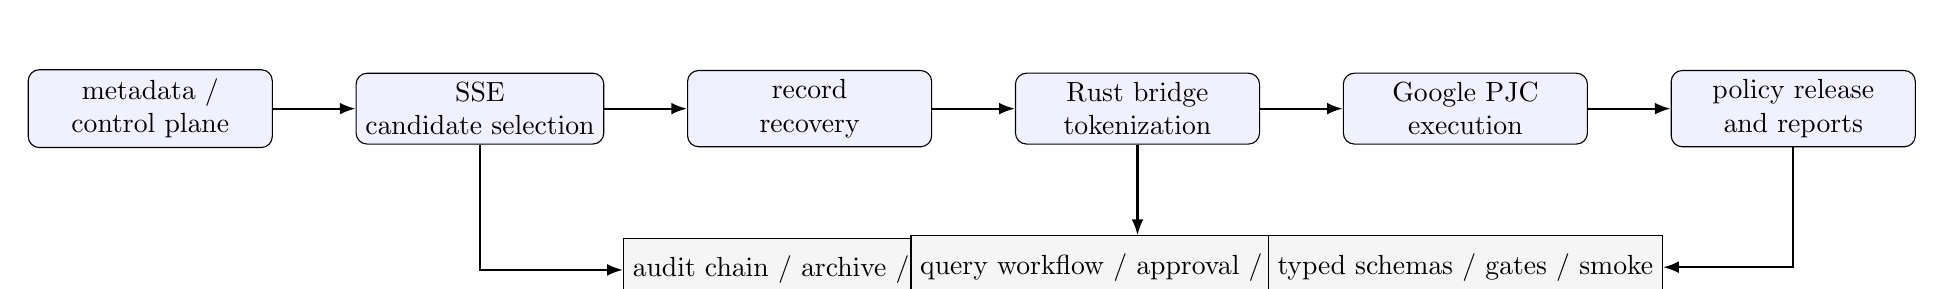
\begin{tikzpicture}[
  node distance=1.05cm,
  stage/.style={rectangle,rounded corners,draw=black,fill=blue!6,minimum width=3.1cm,minimum height=0.9cm,align=center},
  side/.style={rectangle,draw=black,fill=gray!8,minimum width=3.4cm,minimum height=0.8cm,align=center},
  arrow/.style={-{Latex[length=2mm]},thick}
]
  \node[stage] (meta) {metadata /\\control plane};
  \node[stage,right=of meta] (sse) {SSE\\candidate selection};
  \node[stage,right=of sse] (rr) {record\\recovery};
  \node[stage,right=of rr] (bridge) {Rust bridge\\tokenization};
  \node[stage,right=of bridge] (pjc) {Google PJC\\execution};
  \node[stage,right=of pjc] (release) {policy release\\and reports};

  \draw[arrow] (meta) -- (sse);
  \draw[arrow] (sse) -- (rr);
  \draw[arrow] (rr) -- (bridge);
  \draw[arrow] (bridge) -- (pjc);
  \draw[arrow] (pjc) -- (release);

  \node[side,below=1.15cm of rr] (audit) {audit chain / archive / verify};
  \node[side,below=1.15cm of bridge] (workflow) {query workflow / approval / budget};
  \node[side,below=1.15cm of pjc] (schemas) {typed schemas / gates / smoke};

  \draw[arrow] (sse.south) |- (audit.west);
  \draw[arrow] (bridge.south) -- (workflow.north);
  \draw[arrow] (release.south) |- (schemas.east);
\end{tikzpicture}
\caption{平台主链路与治理侧能力}
\label{fig:arch}
\end{figure}

\section{模块划分}

\begin{longtable}{p{0.24\textwidth}p{0.68\textwidth}}
\toprule
\textbf{模块/目录} & \textbf{职责说明} \\
\midrule
\filepath{sse/} & 密文检索、候选导出、legacy demo 接口、SSE 相关策略与样例。 \\
\filepath{services/record_recovery/} & encrypted record store、最小字段恢复、服务边界、authz、health、metrics。 \\
\filepath{bridge/} & join key 规范化、HMAC token 化、PJC 输入准备、bridge job metadata。 \\
\filepath{a-psi/} & Google PJC 集成、PJC 包装、结果发布、策略审计。 \\
\filepath{scripts/} & workflow、release gate、governance、sidecar API、archive、benchmark、smoke。 \\
\filepath{migrations/metadata/} & metadata/control-plane 数据库迁移，包括 workflow、policy、permissions、key registry 等。 \\
\filepath{schemas/} & 所有 verifier-facing typed contract。 \\
\filepath{docs/} & 架构、安全、叙事、治理、runbook、协作和评审材料。 \\
\bottomrule
\end{longtable}

\section{设计原则}

\begin{enumerate}
  \item \textbf{最小必要暴露：} 不让原始 join key 直接进入交互式外部链路。
  \item \textbf{分阶段治理：} SSE、recovery、bridge、PJC、release 各自有边界和审计。
  \item \textbf{typed contract：} 关键产物必须有 schema，而不是随意 JSON。
  \item \textbf{fail closed：} 对高风险路径优先拒绝，而不是默认放行。
  \item \textbf{可验证证据：} 不只输出结果，还要输出 verifier-facing evidence。
\end{enumerate}

\chapter{关键模块实现}

\section{SSE 模块}

\subsection{角色与职责}

SSE 模块承担两项核心职责：

\begin{enumerate}
  \item 在加密存储上完成可搜索检索，得到候选集合；
  \item 在 caller、tenant、dataset、service 等策略约束下导出 bridge 所需候选记录。
\end{enumerate}

\subsection{为何 SSE 是核心而非附属}

本项目不是“先把明文数据都准备好再丢给 PJC”。  
SSE 的意义在于：在进入交集计算之前，先把数据范围缩小到业务允许的候选集合，
减少不必要的暴露面。

\subsection{当前边界}

\begin{itemize}
  \item 保留：candidate selection 核心能力；
  \item 退休：legacy SSE WebSocket 生产暴露面；
  \item 现状：生产模式下 legacy 接口 fail closed，不再作为推荐 query surface。
\end{itemize}

\section{Record Recovery 模块}

\subsection{设计动机}

PJC 不能直接消费 SSE 内部加密记录库，必须先有一个“受控记录恢复”层，将候选集合映
射成 bridge-ready row。该层的目标不是“恢复所有明文”，而是恢复最小必要字段。

\subsection{关键能力}

\begin{enumerate}
  \item encrypted record store；
  \item candidate-bound recovery；
  \item Unix socket / HTTP / mTLS 访问边界；
  \item caller/tenant/dataset/service 绑定；
  \item rate limit、health、audit、metrics。
\end{enumerate}

\section{Rust Bridge 模块}

\subsection{核心职责}

bridge 是项目里非常关键的一层，它连接了“业务数据恢复”与“隐私计算输入”：

\begin{enumerate}
  \item join key 规范化；
  \item HMAC token 化；
  \item 生成 PJC 所需的 server/client CSV；
  \item 生成 job metadata 和 input commitment。
\end{enumerate}

\subsection{安全意义}

bridge 并不是简单格式转换。它承担了：

\begin{itemize}
  \item 原始标识到 token 的边界收敛；
  \item input commitment；
  \item source truthfulness 和 release governance 的绑定入口。
\end{itemize}

\section{Google PJC 模块}

\subsection{项目中的作用}

Google PJC 是当前系统的核心计算引擎，负责两方 token 集合上的交集统计和聚合。  
项目仓库的重点不是重写其协议，而是围绕它建立：

\begin{enumerate}
  \item workflow；
  \item evidence merge；
  \item release binding；
  \item public two-host evidence；
  \item protocol claim boundary。
\end{enumerate}

\subsection{当前能力边界}

应严格表述为：

\begin{quote}
当前 PJC 计算边界是 \texttt{semi-honest/operator-controlled}。
\end{quote}

这意味着系统假设参与方按协议流程执行，但不应宣称已经达到恶意参与方安全。

\section{Policy Release 与 Governance}

\subsection{为什么需要 release gate}

PJC 原始结果不是天然可公开结果。  
系统必须回答：

\begin{enumerate}
  \item 结果是否达到最小阈值；
  \item 是否存在重复查询或 near-duplicate query；
  \item 结果是否绑定到正确输入和正确审批；
  \item 是否可以发布为 public report。
\end{enumerate}

\subsection{当前实现}

当前 release 治理已经包括：

\begin{itemize}
  \item \texttt{release\_policy\_gate/v1}
  \item \texttt{source\_export\_manifest/v1}
  \item \texttt{source\_attestation/v1}
  \item \texttt{source\_truthfulness\_report/v1}
  \item \texttt{release\_governance\_report/v1}
  \item privacy budget ledger
  \item approval flow
  \item public/operator report separation
\end{itemize}

\section{Metadata / Control Plane}

\subsection{控制面数据库的角色}

这里的“数据库”不是完整电商业务库，而是两类东西：

\begin{enumerate}
  \item metadata/control-plane 状态库；
  \item encrypted record store。
\end{enumerate}

metadata sidecar 负责：

\begin{itemize}
  \item tenant / dataset / caller / service；
  \item workflow submissions；
  \item permissions / policy / audit；
  \item privacy budget；
  \item key registry / identity mapping。
\end{itemize}

\section{Query Workflow 与 Operator Surface}

\subsection{Query Workflow}

系统不是“跑一个 shell 脚本就算查询完成”，而是有明确的 workflow：

\begin{enumerate}
  \item request
  \item submit / dry-run / enqueue
  \item worker claim / execute
  \item release gate
  \item archive / status / public summary
\end{enumerate}

\subsection{Operator Dashboard}

operator surface 不是纯展示页，而是承担：

\begin{itemize}
  \item request workflow
  \item approval
  \item release visibility
  \item audit/public summary
  \item deployment evidence aggregation
\end{itemize}

\chapter{安全设计与威胁模型}

\section{威胁模型概览}

本项目当前明确区分两类问题：

\begin{enumerate}
  \item \textbf{protocol-internal 问题：}
  恶意协议偏离、active-secure/malicious-secure 缺失、更强的 SSE 泄露模型缓解。
  \item \textbf{protocol-external / governance 问题：}
  source truthfulness、release legitimacy、审批、审计、外部锚点、operator-side trust root。
\end{enumerate}

\section{当前已经解决得比较好的部分}

\begin{itemize}
  \item legacy SSE 生产退休
  \item input commitment
  \item source attestation / release governance
  \item privacy budget / duplicate / overlap 治理
  \item audit chain / seal / archive
  \item caller-safe summary / session / headers / redaction
\end{itemize}

\section{当前明确承认的边界}

\begin{enumerate}
  \item PJC 不是 malicious-secure；
  \item source truthfulness 目前属于治理闭环，不是密码学证明；
  \item 外部 immutable trust root、enterprise identity/KMS、HA/SRE 仍属于 operator-side 问题。
\end{enumerate}

\section{为什么不能过度宣称}

当前项目最容易被误解的地方在于：

\begin{itemize}
  \item 顶层 live closure 全绿，并不等于 malicious-secure；
  \item typed evidence 完整，并不等于企业 trust-root 完整；
  \item governance 做得强，并不等于协议对恶意参与方已经给出密码学级防护。
\end{itemize}

\chapter{电商叙事环境与平台价值}

\section{为什么电商场景重要}

本项目并不是随意套了一个行业场景。电商环境的重要性在于：

\begin{enumerate}
  \item 它天然包含订单、归因、支付、履约、客服等跨角色、多租户、多数据域问题；
  \item 它要求系统同时处理隐私查询、权限治理、审批发布和审计追责；
  \item 它能证明项目不是孤立协议实验，而是有业务约束的平台实现。
\end{enumerate}

\section{项目中的电商适配内容}

\begin{itemize}
  \item 订单/归因/支付/履约/客服事实层；
  \item business identity 角色；
  \item business access / mask / deny；
  \item fact import；
  \item logistics rollout；
  \item console workbench；
  \item request / approval / workflow。
\end{itemize}

\section{应避免的误读}

不应把本项目说成：

\begin{itemize}
  \item 完整电商业务平台；
  \item 完整 customer 360 数仓；
  \item 完整企业级多租户运营后台。
\end{itemize}

它更准确的说法是：

\begin{quote}
一个面向电商隐私分析场景的 \textbf{SSE + PJC} 平台化实现。
\end{quote}

\chapter{项目验证与当前状态}

\section{验证体系}

项目验证不是单一测试，而是多层证据：

\begin{enumerate}
  \item JSON schema contract
  \item smoke / negative tests
  \item CI checks
  \item typed report / gate
  \item module-level live evidence archive
  \item top-level production closure gate
\end{enumerate}

\section{当前 authoritative 状态}

当前顶层 authoritative 结论可概括为：

\begin{itemize}
  \item 顶层模块数：16
  \item repo-side：全部通过
  \item live evidence：全部通过
  \item remaining live blockers：0
\end{itemize}

这一结果说明：项目已经把 verifier-facing 的工程与证据层做到很完整。  
但它不应被误读成“协议级恶意安全已经解决”。

\section{客观评价}

可以将当前项目状态概括为：

\begin{quote}
这是一个工程完成度很高、平台化明显、证据链完整的
\textbf{SSE + Google PJC} 比赛作品。
它最强的是平台治理、typed contract 与 verifier-facing 收口；
它最需要克制的是 malicious-secure 安全声明。
\end{quote}

\chapter{局限性与后续工作}

\section{当前局限性}

\begin{enumerate}
  \item PJC 仍然停留在 \texttt{semi-honest/operator-controlled} 边界；
  \item 更强的 oracle / differencing 攻击仅被缓解，没有理论根治；
  \item SSE 的更强泄露模型缓解未完成；
  \item 企业级 immutable anchor、identity/KMS lifecycle、HA/SRE 仍属于外部 trust-root。
\end{enumerate}

\section{后续工作分类}

\subsection{不更换协议仍可继续增强的方向}

\begin{itemize}
  \item 更严格的 source attestation 和 signed signoff
  \item 更严格的 release gate
  \item 更强的 privacy budget / overlap / abuse heuristics
  \item 更严格的 plaintext boundary 和 workflow 治理
\end{itemize}

\subsection{必须改变协议或外部 trust-root 才能真正解决的方向}

\begin{itemize}
  \item active-secure / malicious-secure backend
  \item source/value cryptographic proof
  \item ORAM / forward-private SSE 等更强泄露缓解
  \item 真实 enterprise trust-root 托管与长期运行
\end{itemize}

\chapter{结论}

本文围绕一个面向电商隐私分析场景的隐私计算平台，系统介绍了其总体设计、关键模块、
治理体系、安全边界和当前状态。项目当前的核心贡献不只是“把 SSE 和 PJC 跑通”，更
在于围绕这条主链实现了 control-plane、workflow、release governance、privacy budget、
audit chain、typed schema、verifier-facing evidence 等平台能力。

从客观角度看，该项目已经具备较高的工程完整度和答辩价值，能够支撑“不是协议玩具，
而是平台化作品”的评价；但同时也必须严格承认，其协议边界仍然是
\texttt{semi-honest/operator-controlled}，因此不能夸大为 malicious-secure 的
生产级终态系统。

\appendix

\chapter{可替换信息清单}

提交前建议替换以下内容：

\begin{enumerate}
  \item 封面中的作者、指导教师、学校、日期
  \item 摘要中的字数、措辞和关键词
  \item 当前 authoritative 数字，如模块数、live 状态
  \item 若有真实截图、流程图、部署图，可插入 \verb|\includegraphics|
  \item 若学校有固定格式，可替换页眉、标题页和章节样式
\end{enumerate}

\chapter{建议插图位置}

\begin{enumerate}
  \item 总体架构图
  \item query workflow / approval 流程图
  \item source attestation / release governance 绑定图
  \item module-level live evidence / top-level closure 截图
  \item console / operator dashboard 示例截图
\end{enumerate}

\end{document}
